\documentclass[aspectratio=169]{beamer}

\usetheme{default}
\usefonttheme{professionalfonts}
\setbeamertemplate{navigation symbols}{}
\setbeamertemplate{itemize items}[circle]
\setbeamercolor{itemize item}{fg=white}

\setbeamerfont{title}{series=\bfseries, size=\normalfont\Large}
\setbeamercolor{title}{fg=white}

\setbeamerfont{author}{size=\normalfont\small}
\setbeamercolor{author}{fg=white}

\setbeamerfont{frametitle}{series=\bfseries, size=\normalfont}
\setbeamercolor{frametitle}{fg=white}

\setbeamerfont{framesubtitle}{size=\normalfont\large}
\setbeamercolor{framesubtitle}{fg=white}

\setbeamercolor{background canvas}{bg=black}
\setbeamercolor{normal text}{fg=white}

\setbeamercolor{local structure}{fg=white}

\usepackage[utf8]{inputenc}
\usepackage[english]{babel}
\usepackage{amsmath, amssymb}
\usepackage{amsfonts}
\usepackage{amssymb}
\usepackage{graphicx}
\usepackage[]{bm}
\usepackage[]{multimedia}
\usepackage[]{multicol}
\usepackage[squaren,Gray]{SIunits}
\usepackage[]{nicefrac}

\graphicspath{{imgs/}}

\DeclareMathOperator*{\minimize}{minimize}
\DeclareMathOperator*{\maximize}{maximize}
\DeclareMathOperator*{\subjectto}{subject~to}


\usepackage{tikz} % Required for drawing custom shapes
\usetikzlibrary{shapes.geometric, math, positioning, calc, patterns, angles, quotes}
\usetikzlibrary{patterns.meta,decorations.pathmorphing}

\usepackage{circuitikz}
\ctikzset{bipoles/thickness=1.2}

\newcommand{\midlabelline}[3]{
  \node (midlabel) at ($ (#1)!.5!(#2) $) {#3};
  \draw[latex-] (#1) --  (midlabel);
  \draw[-latex] (midlabel) -- (#2);
}

\usepackage{pgfplots}
\pgfplotsset{compat=newest}
\usepgfplotslibrary{fillbetween, groupplots}

%\usepackage[]{listings}
\usepackage[many]{tcolorbox}
\tcbuselibrary{listings}

%% \definecolor{codegreen}{rgb}{0,0.8,0}
%% \definecolor{codegray}{rgb}{0.5,0.5,0.5}
%% %\definecolor{codepurple}{rgb}{0.58,0,0.82}
%% \definecolor{codepurple}{rgb}{0,0.8,0}
%% \definecolor{backcolour}{rgb}{0.0, 0.0, 0.0}

\definecolor{codegreen}{rgb}{0,0.6,0}
\definecolor{codered}{rgb}{0.6,0.1,0}
\definecolor{codegray}{rgb}{0.5,0.5,0.5}
\definecolor{codepurple}{rgb}{0.58,0,0.82}
\definecolor{backcolour}{rgb}{0, 0, 0}
\definecolor{lightgray}{gray}{0.95}
\definecolor{codeblue}{rgb}{0.117,0.403,0.713}

\newcounter{ipythcntr}
\renewcommand{\theipythcntr}{\texttt{[\arabic{ipythcntr}]}}
\newcommand{\ipin}[1][]{
  \stepcounter{ipythcntr}
  \hspace{-10pt}
  \color{codeblue}In  \theipythcntr}
\newcommand{\ipout}[1][\theipythcntr]{
  \hspace{-10pt}
  \color{codered}Out \theipythcntr}

\lstdefinestyle{mystyle}{
  language=Python,
  moredelim=[is][\ipin]{In[}{]},
  moredelim=[is][\ipout]{Out[}{]},
  backgroundcolor=\color{backcolour},
  commentstyle=\color{codegreen},
  keywordstyle=\color{magenta},
  numberstyle=\tiny\color{codegray},
  stringstyle=\color{codepurple},
  basicstyle=\ttfamily\footnotesize,
  breakatwhitespace=false,
  breaklines=true,
  captionpos=b,
  keepspaces=true,
  numbers=left,
  numbersep=5pt,
  showspaces=false,
  showstringspaces=false,
  showtabs=false,
  tabsize=2,
}

\lstset{style=mystyle}

\usepackage[]{stanli}

\title{Driven oscillators and the resonance phenomenon}
\author{Jean-Christophe LOISEAU}
\institute{Arts \& Métiers Institute of Technology, January 2022}
\date{}

\begin{document}

\frame{\titlepage}

{
  \setbeamercolor{background canvas}{bg=white}
  \begin{frame}
    \centering

    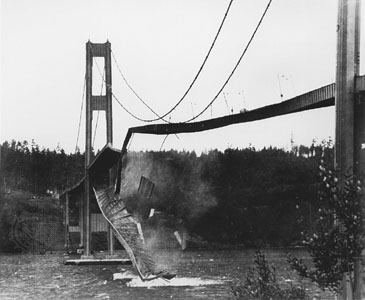
\includegraphics[height=.8\textheight]{tacoma_bridge}

    {
      \color{black}
      Collapse of the Tacoma bridge (1940).
    }
    
  \end{frame}

  \begin{frame}
    \vfill
    \begin{minipage}{.48\textwidth}
      \centering
      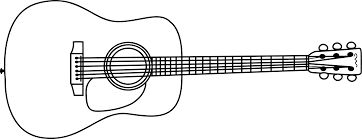
\includegraphics[width=\textwidth]{guitar}
    \end{minipage}%
    \hfill
    \begin{minipage}{.48\textwidth}
      \centering
      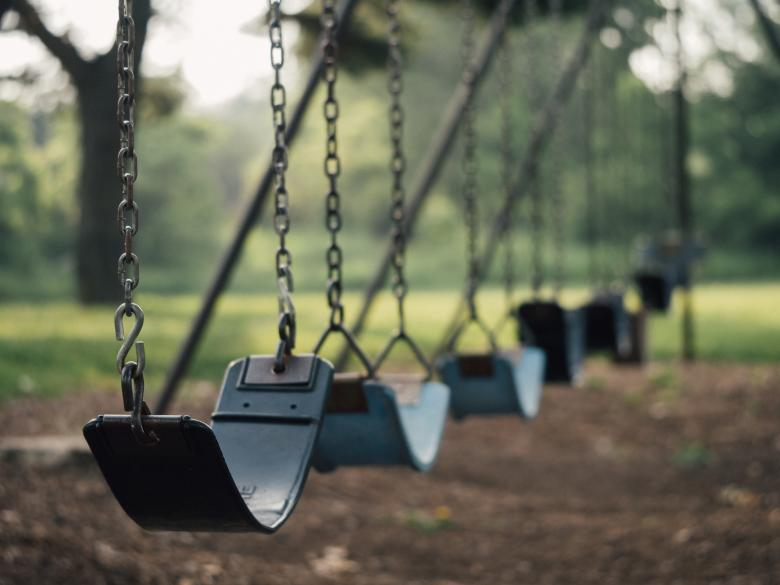
\includegraphics[width=\textwidth]{balancoire}
    \end{minipage}
    \vfill
  \end{frame}
}


\begin{frame}
  \vfill
  \centering
  \large

  \underline{Forced Liénard equation}

  \[
  \ddot{x} + f(x) \dot{x} + g(x) = \gamma \cos(\omega t)
  \]

  \vfill
\end{frame}

\begin{frame}
  \vfill
  \centering
  \large

  \underline{Forced Harmonic oscillator}

  \[
  \ddot{x} + 2\xi \dot{x} + x = \gamma \cos(\omega t)
  \]

  \vfill
\end{frame}

{
  \setbeamercolor{background canvas}{bg=white}
  \begin{frame}
    \hfill
    \begin{circuitikz}
		  % Circuit
		  \draw[black, line width=0.8]
      
		  (1,6) to [sinusoidal voltage source, l_=$V_S$, i=$I$] (1,1)
		  (1,6) to [resistor, l_=$R$] ++(5,0) to [inductor, l_=$L$] ++(0,-5) to [capacitor, l_=$C$] +(-5,0) ;
		  
		  % Voltage Infos
		  \midlabelline{2,8}{8,8}{$V_R$}
		  \midlabelline{9,7}{9,1}{$V_L$}
		  \midlabelline{2,0}{8,0}{$V_C$}
		  
		  % Grid
      %\draw[help lines] (0,0) grid (7,7)	;
	  \end{circuitikz}
    \hfill
  \end{frame}
}

\begin{frame}[t, c]{Forced linear oscillator (no damping)}{}
  \vfill
  \begin{minipage}{.48\textwidth}
    \large
    \begin{overprint}
      \onslide<1>
      \[
      \ddot{x} + x = \gamma \cos(\omega t)
      \]

      \onslide<2>
      \[
      \ddot{z} + z = \gamma e^{i\omega t}
      \]

      \onslide<3>
      \[
      \left( 1-\omega^2 \right) \hat{z} e^{i\varphi} = \gamma
      \]

      \onslide<4>
      \[
      \hat{z} = \dfrac{\gamma}{1 - \omega^2} e^{-i\varphi}
      \]
    \end{overprint}
  \end{minipage}%
  \hfill
  \begin{minipage}{.48\textwidth}
    \centering
    \onslide<4>
    \begin{tikzpicture}[>=stealth]
      \begin{axis}[
          xmin=0, xmax=2,
          ymin=0, ymax=10,
          restrict y to domain=0:10,
          xlabel={Forcing frequency $\omega$}, ylabel={$\vert \hat{z}(\omega) \vert$},
          width=\textwidth,
          axis lines = middle,
          axis line style = {->},
          x label style={at={(axis description cs:0.5,-0.1)},anchor=north},
          y label style={at={(axis description cs:-0.075,.5)},rotate=90,anchor=south},
          no markers,
          ytick style={draw=none},
          yticklabels=\empty,
        ]

        \addplot[domain=0:0.999, samples=256, color=orange, ultra thick] { 1 / sqrt( (1-x^2)^2 ) };
        \addplot[domain=1.01:2, samples=128, color=orange, ultra thick] { 1 / sqrt( (1-x^2)^2 ) };

        \addplot[domain=0:2, dashed] coordinates {(1, 0)(1, 10)};

      \end{axis}
    \end{tikzpicture}
  \end{minipage}
  \vfill
\end{frame}

{
  \setbeamercolor{background canvas}{bg=white}
  \setbeamercolor{normal text}{fg=black}
  \usebeamercolor[fg]{normal text}

  \begin{frame}[fragile]{}{}
    \vfill
    \centering

    \begin{tikzpicture}[>=stealth]
      \begin{axis}[
          xmin=0, xmax=50,
          ymin=-2, ymax=2,
          xlabel={$t$}, ylabel={$x(t)$},
          width=.9\textwidth, height=.75\textheight,
          axis lines = middle,
          axis line style = {->},
          x label style={at={(axis description cs:1.025,0.5)},anchor=north},
          y label style={at={(axis description cs:-0.025,.5)},rotate=90,anchor=south},
          no markers,
          xtick style={draw=none},
          xticklabels=\empty,
          ytick style={draw=none},
          yticklabels=\empty,
        ]

        \addplot[domain=0:50, samples=512, color=red, ultra thick] {x * sin(deg(x)) / 25};
      \end{axis}
    \end{tikzpicture}
    \vfill
  \end{frame}
}

\begin{frame}[t, c]{Forced linear oscillator (linear damping)}{}
  \vfill
  \begin{minipage}{.48\textwidth}
    \large
    \begin{overprint}
      \onslide<1>
      \[
      \ddot{x} + 2\xi \dot{x} + x = \gamma \cos(\omega t)
      \]

      \onslide<2>
      \[
      \ddot{z} + 2\xi \dot{z} + z = \gamma e^{i\omega t}
      \]

      \onslide<3>
      \[
      \left( 2\xi i\omega + 1-\omega^2 \right) \hat{z} e^{i\varphi} = \gamma
      \]

      \onslide<4>
      \[
      \hat{z} = \dfrac{\gamma}{2\xi i\omega + 1 - \omega^2} e^{-i\varphi}
      \]
    \end{overprint}
  \end{minipage}%
  \hfill
  \begin{minipage}{.48\textwidth}
    \centering
    \onslide<4>
    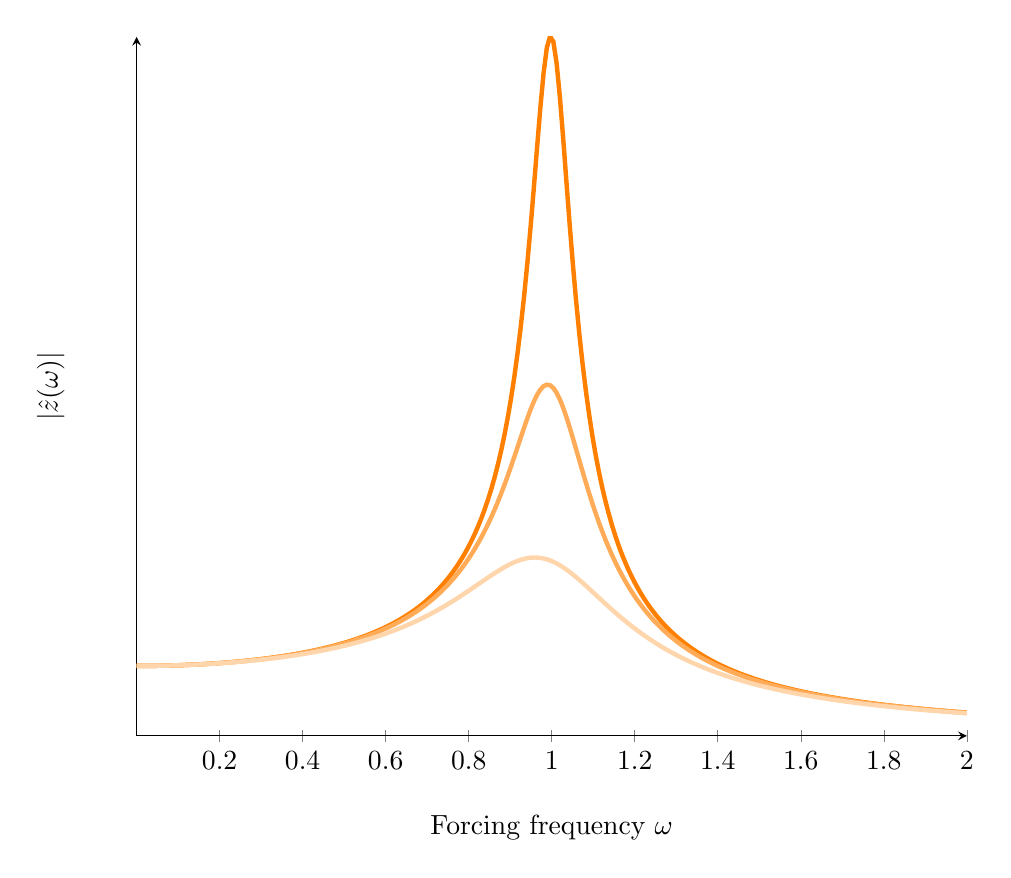
\begin{tikzpicture}[>=stealth]
      \begin{axis}[
          xmin=0, xmax=2,
          ymin=0, ymax=10,
          restrict y to domain=0:12,
          xlabel={Forcing frequency $\omega$}, ylabel={$\vert \hat{z}(\omega) \vert$},
          width=\textwidth,
          axis lines = middle,
          axis line style = {->},
          x label style={at={(axis description cs:0.5,-0.1)},anchor=north},
          y label style={at={(axis description cs:-0.075,.5)},rotate=90,anchor=south},
          no markers,
          ytick style={draw=none},
          yticklabels=\empty,
        ]

        \addplot[domain=0:2, samples=256, color=gray, color=orange!100, ultra thick] { 1 / sqrt( (1-x^2)^2  + (2*0.05*x)^2 ) };

        \addplot[domain=0:2, samples=256, color=gray, color=orange!66, ultra thick] { 1 / sqrt( (1-x^2)^2  + (2*0.1*x)^2 ) };

        \addplot[domain=0:2, samples=256, color=gray, color=orange!33, ultra thick] { 1 / sqrt( (1-x^2)^2  + (2*0.2*x)^2 ) };

      \end{axis}
    \end{tikzpicture}
  \end{minipage}
  \vfill
\end{frame}


\begin{frame}[t, c]{Conservative nonlinear oscillator}{}
  \vfill
  \centering
  \large

  \underline{Forced Liénard equation}

  \[
  \ddot{x} + g(x) = \gamma \cos(\omega t)
  \]

  \vfill
\end{frame}

\begin{frame}[t, c]{Conservative nonlinear oscillator}{}
  \vfill
  \centering
  \large

  \underline{Forced Duffing oscillator}

  \[
  \ddot{x} + x + \epsilon x^3 = \gamma \cos(\omega t)
  \]

  \vfill
\end{frame}

\begin{frame}[t, c]{Conservative nonlinear oscillator}{}
  \vfill
  \large
  \[
  \dfrac{d^2 x}{d\tau^2} + \dfrac{1}{\omega^2} x + \dfrac{\epsilon}{\omega^2} x^3 = \dfrac{\gamma}{\omega^2}\cos(\tau)
  \]
  \vfill
\end{frame}


\begin{frame}[t, c]{Conservative nonlinear oscillator}{}
  \vfill
  \large

  Retaining only terms of order $\mathcal{O}(\epsilon)$ leads to

  \[
  \dfrac{d^2 x}{d\tau^2} +  x  = \epsilon \left( \Gamma \cos(\tau) +2\omega_1 x - x^3  \right)
  \]

  \medskip

  where the parameters are defined as \(\gamma = \epsilon \Gamma \).
  \vfill
\end{frame}

\begin{frame}[t, c]{Conservative nonlinear oscillator}{}
  \vfill
  \large
  Introducing the power series expansion $x(\tau, \epsilon) = x_0(\tau) + \epsilon x_1(\tau)$ yields

  \[
  \begin{aligned}
    \mathcal{O}(1) : & \quad \ddot{x}_0 + x_0 = 0 \\
    \mathcal{O}(\epsilon) : & \quad \ddot{x}_1 + x_1 = 2\omega_1 x_0 - x_0^3 + \Gamma \cos(\tau)
  \end{aligned}
  \]

  which we can now solve.
  \vfill
\end{frame}

\begin{frame}[t, c]{Conservative nonlinear oscillator}{}
  \vfill
  \large
  At leading order, the solution is given by $x_0(\tau) = A \cos(\tau)$.
  At the next order, we have

  \[
  \ddot{x}_1 + x_1 = \underbrace{\left( 2 \omega_1 A - \dfrac{3}{4} A^3 + \Gamma \right)}_{=0} \cos(\tau) - \dfrac{A^3}{4} \cos(3\tau)
  \]

  which leads to $\omega_1 = \dfrac{3}{8} A^2 - \dfrac{\Gamma}{2A}$ to avoid secular growth.

  \vfill
\end{frame}

\begin{frame}[t, c]{Conservative nonlinear oscillator}{}
  \vfill
  \large
  \begin{minipage}{.48\textwidth}
    In the original variables, this leads to

    \[
    \dfrac{3}{4} \epsilon A^3 + \left(1 - \omega^2 \right) A - \gamma = 0
    \]

    \medskip

    describing the \alert{\textbf{nonlinear response function}} of the system.
  \end{minipage}%
  \hfill
  \begin{minipage}{.48\textwidth}
    \centering
    \begin{tikzpicture}[>=stealth]
      \begin{axis}[
          xmin=0, xmax=2,
          ymin=0, ymax=10,
          restrict y to domain=0:10,
          xlabel={Forcing frequency $\omega$}, ylabel={$\vert A(\omega) \vert$},
          width=\textwidth,
          axis lines = middle,
          axis line style = {->},
          x label style={at={(axis description cs:0.5,-0.1)},anchor=north},
          y label style={at={(axis description cs:-0.075,.5)},rotate=90,anchor=south},
          no markers,
          ytick style={draw=none},
          yticklabels=\empty,
        ]


        \addplot[smooth, orange, ultra thick] table[x=x, y=y]{data/first_root_conservative.dat};
        \addplot[smooth, orange, ultra thick] table[x=x, y=y]{data/second_root_conservative.dat};
        \addplot[smooth, orange, ultra thick, dashed] table[x=x, y=y]{data/third_root_conservative.dat};
      \end{axis}
    \end{tikzpicture}
  \end{minipage}

  \vfill
\end{frame}


\begin{frame}[t, c]{Conservative nonlinear oscillator}{}
  \vfill
  \large
  \begin{minipage}{.48\textwidth}
    Nonlinearity prevents the unbounded growth of the oscillations by generating higher-order harmonics.

    \bigskip

    As the amplitude grows, the resonant forcing frequency changes.
  \end{minipage}%
  \hfill
  \begin{minipage}{.48\textwidth}
    \centering
    \begin{tikzpicture}[>=stealth]
      \begin{axis}[
          xmin=0, xmax=2,
          ymin=0, ymax=10,
          restrict y to domain=0:10,
          xlabel={Forcing frequency $\omega$}, ylabel={$\vert A(\omega) \vert$},
          width=\textwidth,
          axis lines = middle,
          axis line style = {->},
          x label style={at={(axis description cs:0.5,-0.1)},anchor=north},
          y label style={at={(axis description cs:-0.075,.5)},rotate=90,anchor=south},
          no markers,
          ytick style={draw=none},
          yticklabels=\empty,
        ]

        \addplot[smooth, orange, ultra thick] table[x=x, y=y]{data/first_root_conservative.dat};
        \addplot[smooth, orange, ultra thick] table[x=x, y=y]{data/second_root_conservative.dat};
        \addplot[smooth, orange, ultra thick, dashed] table[x=x, y=y]{data/third_root_conservative.dat};
        
      \end{axis}
    \end{tikzpicture}
  \end{minipage}
 
  \vfill
\end{frame}



\begin{frame}[t, c]{Dissipative nonlinear oscillator}{}
  \vfill
  \large
  \centering

  \underline{Forced Duffing oscillator with damping}

  \[
  \ddot{x} + \delta \dot{x} + x + \epsilon x^3 = \gamma \cos(\omega t)
  \]

  \vfill
\end{frame}

\begin{frame}[t, c]{Dissipative nonlinear oscillator}{}
  \vfill
  \large

  Let's illustrate another technique to derive the nonlinear response function, namely \textbf{\alert{Harmonic Balance}}.
  Assume the solution is of the form $x(t) = A \cos(\omega t) + B \sin(\omega t)$ and inject into the equations.

  \vfill
\end{frame}

\begin{frame}[t, c]{Dissipative nonlinear oscillator}{}
  \vfill
  \large

  \[
  \begin{aligned}
    & \left( -\omega^2 A + \omega \delta B + A + \dfrac{3}{4} \epsilon A^3 + \dfrac{3}{4} \epsilon AB^2 - \gamma \right) \cos(\omega t) \\
    & + \left( -\omega^2 B - \omega \delta A + \dfrac{3}{4} \epsilon B^3 + B + \dfrac{3}{4} \epsilon A^2 B \right) \sin(\omega t) \\
    & + \left( \dfrac{1}{4} \epsilon A^3 - \dfrac{3}{4} \epsilon AB^3 \right) \cos(3\omega t) \\
    & + \left( \dfrac{3}{4} \epsilon A^2 B - \dfrac{1}{4} \epsilon B^3 \right) \sin(3\omega t) = 0
  \end{aligned}
  \]

  \vfill
\end{frame}

\begin{frame}[t, c]{Dissipative nonlinear oscillator}{}
  \vfill
  \large

  Neglecting superharmonics at $3 \omega$ leads to the balance equations

  \[
  \begin{aligned}
    \left(1 - \omega^2 \right) A + \omega \delta B + \dfrac{3}{4} \epsilon A^3 + \dfrac{3}{4} \epsilon A B^2 & = \gamma \\
    \left( 1 - \omega^2 \right) B - \omega \delta A + \dfrac{3}{4} \epsilon B^3 + \dfrac{3}{4} \epsilon A^2 B & = 0.
  \end{aligned}
  \]

  If $B = 0$ and $\delta = 0$, we recover the response function derived for the undamped case.

  \vfill
\end{frame}

\begin{frame}[t, c]{Dissipative nonlinear oscillator}{}
  \large
  \vfill

  \begin{minipage}{.48\textwidth}
    These conditions can be combined into

    \[
    \left[ \left( \dfrac{3}{4}\epsilon R^2 + 1 - \omega^2 \right)^2 + \left( \delta \omega \right)^2 \right] R^2 = \gamma^2
    \]

    \medskip

    with $R = \sqrt{A^2 + B^2}$ the amplitude of the oscillation.
  \end{minipage}%
  \hfill
  \begin{minipage}{.48\textwidth}
    \begin{tikzpicture}[>=stealth]
      \begin{axis}[
          xmin=0, xmax=2,
          ymin=0, ymax=10,
          restrict y to domain=0:10,
          xlabel={Forcing frequency $\omega$}, ylabel={$\vert R(\omega) \vert$},
          width=\textwidth,
          axis lines = middle,
          axis line style = {->},
          x label style={at={(axis description cs:0.5,-0.1)},anchor=north},
          y label style={at={(axis description cs:-0.075,.5)},rotate=90,anchor=south},
          no markers,
          ytick style={draw=none},
          yticklabels=\empty,
          legend style = {fill=black},
        ]


        \addplot[smooth, orange, ultra thick] table[x=x, y=y]{data/first_root_dissipative_multi.dat};
        \addplot[smooth, orange!50, ultra thick] table[x=x, y=y]{data/first_root_dissipative_single.dat};
        \legend{High-amplitude forcing, Low-amplitude forcing};

        \addplot[smooth, orange, ultra thick, dashed] table[x=x, y=y]{data/second_root_dissipative_multi.dat};
        \addplot[smooth, orange, ultra thick] table[x=x, y=y]{data/third_root_dissipative_multi.dat};

        \addplot[smooth, orange!50, ultra thick] table[x=x, y=y]{data/third_root_dissipative_single.dat};

      \end{axis}
    \end{tikzpicture}
  \end{minipage}

  \vfill
\end{frame}


\begin{frame}[t, c]{Dissipative nonlinear oscillator}{}
  \large
  \vfill

  \begin{minipage}{.48\textwidth}
    It can be simplified to
    
    \[
    \left[ \left( \dfrac{3}{4} R^2 - 2\omega_1 \right)^2 + \Delta^2 \right] R^2 = \Gamma^2
    \]

    \medskip

    with $1 - \omega^2 = -2\epsilon \omega_1$, $\Delta = \nicefrac{\delta}{\epsilon}$ and $\Gamma = \nicefrac{\gamma}{\epsilon}$.
  \end{minipage}%
  \hfill
  \begin{minipage}{.48\textwidth}
    \begin{tikzpicture}[>=stealth]
      \begin{axis}[
          xmin=0, xmax=2,
          ymin=0, ymax=10,
          restrict y to domain=0:10,
          xlabel={Forcing frequency $\omega$}, ylabel={$\vert R(\omega) \vert$},
          width=\textwidth,
          axis lines = middle,
          axis line style = {->},
          x label style={at={(axis description cs:0.5,-0.1)},anchor=north},
          y label style={at={(axis description cs:-0.075,.5)},rotate=90,anchor=south},
          no markers,
          ytick style={draw=none},
          yticklabels=\empty,
          legend style = {fill=black},
        ]


        \addplot[smooth, orange, ultra thick] table[x=x, y=y]{data/first_root_dissipative_multi.dat};
        \addplot[smooth, orange!50, ultra thick] table[x=x, y=y]{data/first_root_dissipative_single.dat};
        \legend{High-amplitude forcing, Low-amplitude forcing};

        \addplot[smooth, orange, ultra thick, dashed] table[x=x, y=y]{data/second_root_dissipative_multi.dat};
        \addplot[smooth, orange, ultra thick] table[x=x, y=y]{data/third_root_dissipative_multi.dat};

        \addplot[smooth, orange!50, ultra thick] table[x=x, y=y]{data/third_root_dissipative_single.dat};

      \end{axis}
    \end{tikzpicture}
  \end{minipage}

  \vfill
\end{frame}


\begin{frame}[t, c]{Dissipative nonlinear oscillator}{}
  \large
  \vfill

  \begin{minipage}{.48\textwidth}
    As $\Gamma$ increases, $R(\omega)$ switches from being single-valued to multi-valued because of a \textbf{\alert{saddle-node bifurcation}}.
  \end{minipage}%
  \hfill
  \begin{minipage}{.48\textwidth}
    \begin{tikzpicture}[>=stealth]
      \begin{axis}[
          xmin=0, xmax=2,
          ymin=0, ymax=10,
          restrict y to domain=0:10,
          xlabel={Forcing frequency $\omega$}, ylabel={$\vert R(\omega) \vert$},
          width=\textwidth,
          axis lines = middle,
          axis line style = {->},
          x label style={at={(axis description cs:0.5,-0.1)},anchor=north},
          y label style={at={(axis description cs:-0.075,.5)},rotate=90,anchor=south},
          no markers,
          ytick style={draw=none},
          yticklabels=\empty,
          legend style = {fill=black},
        ]


        \addplot[smooth, orange, ultra thick] table[x=x, y=y]{data/first_root_dissipative_multi.dat};
        \addplot[smooth, orange!50, ultra thick] table[x=x, y=y]{data/first_root_dissipative_single.dat};
        \legend{High-amplitude forcing, Low-amplitude forcing};

        \addplot[smooth, orange, ultra thick, dashed] table[x=x, y=y]{data/second_root_dissipative_multi.dat};
        \addplot[smooth, orange, ultra thick] table[x=x, y=y]{data/third_root_dissipative_multi.dat};

        \addplot[smooth, orange!50, ultra thick] table[x=x, y=y]{data/third_root_dissipative_single.dat};

      \end{axis}
    \end{tikzpicture}
  \end{minipage}

  \vfill
\end{frame}


\begin{frame}[t, c]{Dissipative nonlinear oscillator}{}
  \large
  \vfill

  \begin{minipage}{.48\textwidth}
    What are the critical values of $\Gamma$ and $\omega_1$ at which this bifurcation happen ?
  \end{minipage}%
  \hfill
  \begin{minipage}{.48\textwidth}
    \begin{tikzpicture}[>=stealth]
      \begin{axis}[
          xmin=0, xmax=2,
          ymin=0, ymax=10,
          restrict y to domain=0:10,
          xlabel={Forcing frequency $\omega$}, ylabel={$\vert R(\omega) \vert$},
          width=\textwidth,
          axis lines = middle,
          axis line style = {->},
          x label style={at={(axis description cs:0.5,-0.1)},anchor=north},
          y label style={at={(axis description cs:-0.075,.5)},rotate=90,anchor=south},
          no markers,
          ytick style={draw=none},
          yticklabels=\empty,
          legend style = {fill=black},
        ]


        \addplot[smooth, orange, ultra thick] table[x=x, y=y]{data/first_root_dissipative_multi.dat};
        \addplot[smooth, orange!50, ultra thick] table[x=x, y=y]{data/first_root_dissipative_single.dat};
        \legend{High-amplitude forcing, Low-amplitude forcing};

        \addplot[smooth, orange, ultra thick, dashed] table[x=x, y=y]{data/second_root_dissipative_multi.dat};
        \addplot[smooth, orange, ultra thick] table[x=x, y=y]{data/third_root_dissipative_multi.dat};

        \addplot[smooth, orange!50, ultra thick] table[x=x, y=y]{data/third_root_dissipative_single.dat};

      \end{axis}
    \end{tikzpicture}
  \end{minipage}

  \vfill
\end{frame}


{
  \setbeamercolor{background canvas}{bg=white}
  \setbeamercolor{normal text}{fg=black}
  \usebeamercolor[fg]{normal text}
  \setbeamercolor{frametitle}{fg=black}
  \setbeamercolor{framesubtitle}{fg=black}

  \setbeamercolor{itemize item}{fg=black}

  \begin{frame}[t, c]{The cusp catastrophe}{\small Forced nonlinear oscillator}

    \centering
    \vfill

    \begin{tikzpicture}[>=stealth]
      \begin{axis}[
          xmin=0, xmax=2,
          ymin=0, ymax=3,
          xlabel={Detuning parameter $\omega_1$}, ylabel={$\Gamma$},
          width=.8\textwidth,
          height=.75\textheight,
          axis lines = middle,
          axis line style = {->},
          x label style={at={(axis description cs:0.5,-0.1)},anchor=north},
          y label style={at={(axis description cs:-0.075,.5)},rotate=90,anchor=south},
          no markers,
          ytick style={draw=none},
          yticklabels=\empty,
          xtick style={draw=none},
          xticklabels=\empty,
        ]

        \draw[dashed] (axis cs:0, 1.432759) -- (axis cs:0.8666, 1.432759) node[below left] {\tiny $\left( \dfrac{\sqrt{3}}{2} \Delta, \sqrt{ \dfrac{32 \sqrt{3} \Delta^3}{27} } \right)$};
        \draw[dashed] (axis cs:0.8666, 1.432759) -- (axis cs:0.8666, 0) node[] {};
        \node[circle, fill=black, inner sep=0pt, minimum size=4pt] at (axis cs: 0.8666, 1.432759) {};

        \addplot[name path=upper, smooth] table[x=x, y=y]{data/cusp_upper_branch.dat};
        \addplot[name path=lower, smooth] table[x=x, y=y]{data/cusp_lower_branch.dat};

        \addplot[orange!50] fill between[of = upper and lower];

      \end{axis}
    \end{tikzpicture}

    \vfill
  \end{frame}


  \begin{frame}[t, c]{The cusp catastrophe}{\small Forced nonlinear oscillator}
    \vfill
    \large

    \begin{minipage}{.48\textwidth}
      The response function is of the form

      \[
      X^3 + p X + q = 0.
      \]

      This is the canonical form of the \textbf{\alert{cusp catastrophe}}.
    \end{minipage}%
    \hfill
    \begin{minipage}{.48\textwidth}
      \centering
      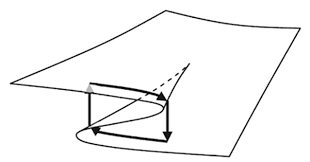
\includegraphics[width=\textwidth]{cusp}
    \end{minipage}

    \vfill
  \end{frame}

  \begin{frame}[t, c]{The cusp catastrophe}{\small Forced nonlinear oscillator}
    \vfill
    \large

    \begin{minipage}{.48\textwidth}
      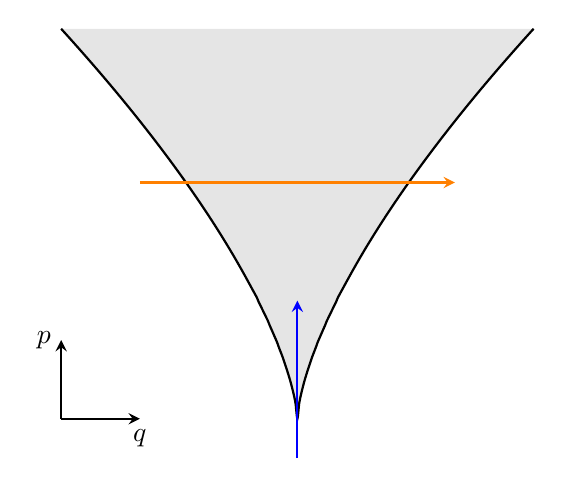
\begin{tikzpicture}[>=stealth]

        \usetikzlibrary{arrows, pgfplots.fillbetween}

        %\draw[help lines] (-3, -1) grid (3, 5);

        \draw[->, thick] (-3, 0) -- (-3, 1) node[left] {$p$};
        \draw[->, thick] (-3, 0) -- (-2, 0) node[below] {$q$};

        \draw[name path=A, domain=-3:3, smooth, thick, fill=gray!20, samples=257] plot (\x, {3*(\x*\x / 2)^(1/3)});

        \draw[->, thick, blue] (0, -0.5) -- (0, 1.5) node[] {};
        \draw[->, thick, orange] (-2, 3) -- (2, 3) node[] {};
      \end{tikzpicture}      
    \end{minipage}%
    \hfill
    \begin{minipage}{.48\textwidth}
      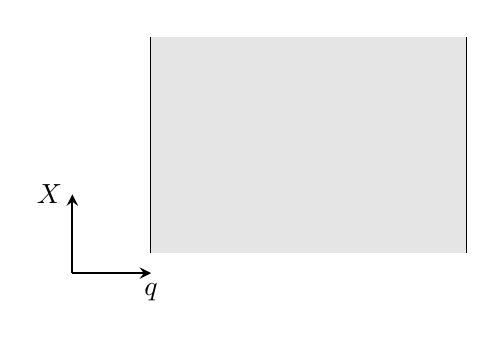
\begin{tikzpicture}[>=stealth]
        %\draw[help lines] (-3, 0) grid (3, 3);

        \draw[->, thick] (-3, 0) -- (-3, 1) node[left] {$X$};
        \draw[->, thick] (-3, 0) -- (-2, 0) node[below] {$q$};

        \draw[-, thick, name path=A] (-2, 0.25) -- (-2, 3) node[] {};
        \draw[-, thick, name path=B] (2, 0.25) -- (2, 3) node[] {};
        \tikzfillbetween[of=A and B] {gray!20};

        \draw[orange, smooth, thick] plot file{data/cusp_saddle_upper.dat};
        \draw[orange, smooth, thick, dashed] plot file{data/cusp_saddle_middle.dat};
        \draw[orange, smooth, thick] plot file{data/cusp_saddle_lower.dat};


      \end{tikzpicture}

      \medskip

      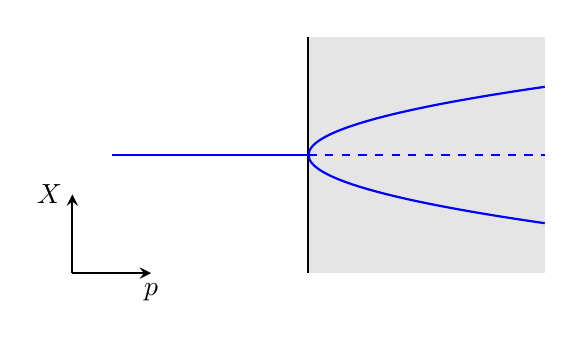
\begin{tikzpicture}[>=stealth]

        \usetikzlibrary{arrows, pgfplots.fillbetween}

        %\draw[help lines] (-3, 0) grid (3, 3);

        \draw[->, thick] (-3, 0) -- (-3, 1) node[left] {$X$};
        \draw[->, thick] (-3, 0) -- (-2, 0) node[below] {$p$};

        \draw[-, thick, name path=A] (0, 0) -- (0, 3) node[] {};
        \draw[white, -, thick, name path=B] (3, 0) -- (3, 3) node[] {};
        \tikzfillbetween[of=A and B] {gray!20};

        \draw[thick, blue] (-2.5, 1.5) -- (0, 1.5) node[] {};
        \draw[thick, dashed, blue] (0, 1.5) -- (3, 1.5) node[] {};
        
        \draw[domain=0:3, smooth, thick, samples=257, blue] plot (\x, {1.5 + 0.5*sqrt(\x)});
        \draw[domain=0:3, smooth, thick, samples=257, blue] plot (\x, {1.5 - 0.5*sqrt(\x)});
      \end{tikzpicture}      
      
    \end{minipage}
    
    \vfill
  \end{frame}

  \begin{frame}[t, c]{The cusp catastrophe}{\small Buckling beam}
    \centering
    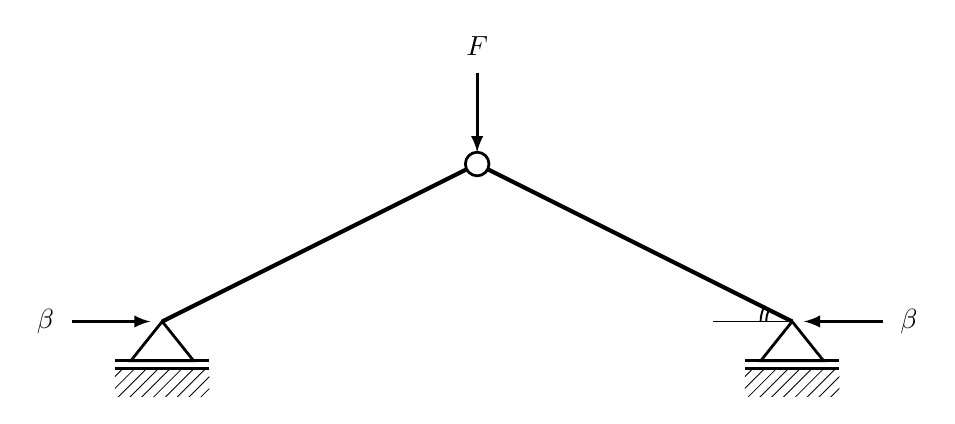
\begin{tikzpicture}[>=stealth]
      %\draw[help lines] (-2,0) grid (10,6);

      \point{a}{0}{2};
      \point{b}{4}{4};
      \point{c}{8}{2};

      \beam{2}{a}{b};
      \beam{2}{b}{c};

      \addon{3}{c}{a}{b}[-1];

      \support{2}{a};
      \hinge{1}{b};
      \support{2}{c};

      \load{1}{a}[180];
      \load{1}{b}[90];
      \load{1}{c};

      \draw[] (8, 2) -- (7, 2) node[] {};
      \node[above] at (4, 5.25) (mass) {$F$};
      \node[left] at (-1.25, 2) (compressions left) {$\beta$};
      \node[right] at (9.25, 2) (compression right) {$\beta$};

    \end{tikzpicture}
  \end{frame}
  
  
  \begin{frame}[t, c]{The cusp catastrophe}{\small Buckling beam}
    \vfill
    \large
    
    \begin{minipage}{.48\textwidth}
      \begin{overprint}
        \onslide<1>
        \centering
        \underline{Total energy in the system}
        
        \[
        V = 2 \mu \theta^2 + F \sin(\theta) - 2\beta \left( 1 - \cos(\theta) \right)
        \]
        
        \onslide<2>
        \underline{Taylor expansion (and $\beta = 2 \mu + b)$}
        
        \[
        V = \dfrac{2\mu + b}{12} \theta^4 - \dfrac{F}{6} \theta^3 - b \theta^2 + m \theta
        \]
        
      \end{overprint}
    \end{minipage}%
    \hfill
    \begin{minipage}{.48\textwidth}
      \centering
      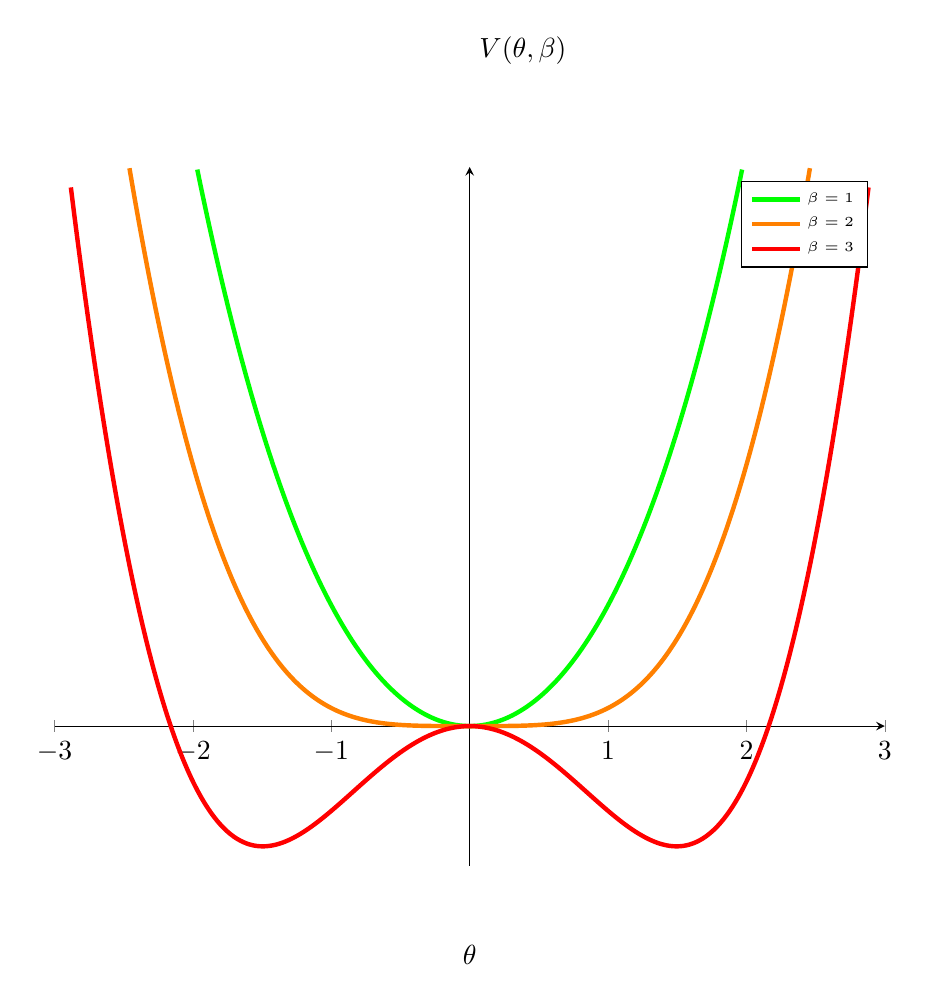
\begin{tikzpicture}[>=stealth]
        \begin{axis}[
            xmin=-3, xmax=3,
            ymin=-1.25, ymax=5,
            restrict y to domain=-2:5,
            xlabel={$\theta$}, ylabel={$V(\theta, \beta)$},
            width=\textwidth,
            axis lines = middle,
            axis line style = {->},
            x label style={at={(axis description cs:0.5,-0.1)},anchor=north},
            y label style={at={(axis description cs:0.5,1.2)}},
            no markers,
            ytick style={draw=none},
            yticklabels=\empty,
          ]
          
          \addplot[domain=-2:2, green, smooth, ultra thick, samples=256] {2*x^2 - 2*( 1 - cos(deg(x)) )};
          
          \addplot[domain=-3:3, orange, smooth, ultra thick, samples=256] {2*x^2 - 4*( 1 - cos(deg(x)) )};
          
          \addplot[domain=-3:3, red, smooth, ultra thick, samples=256] {2*x^2 - 6*( 1 - cos(deg(x)) )};
          
          \legend{\tiny $\beta=1$, \tiny $\beta=2$, \tiny $\beta=3$};
          
        \end{axis}
      \end{tikzpicture}
      
      Potential for $F = 0$
    \end{minipage}
    
    \vfill
  \end{frame}
  
  \begin{frame}[t, c]{The cusp catastrophe}{\small Buckling beam}
    \vfill
    \large
    
    \begin{minipage}{.48\textwidth}
      \centering
      \underline{Equilibria are stationary points}
      
      \[
      \dfrac{2\mu + b}{3} \theta^3 - \dfrac{F}{2} \theta^2 - 2b\theta + F = 0
      \]
    \end{minipage}%
    \hfill
    \begin{minipage}{.48\textwidth}
      \centering
      \begin{tikzpicture}[>=stealth]
        \begin{axis}[
            xmin=-2.5, xmax=2.5,
            ymin=-2, ymax=2,
            xlabel={$F$}, ylabel={$\theta$},
            width=\textwidth,
            axis lines = middle,
            axis line style = {->},
            xtick style={draw=none},
            xticklabels=\empty,
            ytick style={draw=none},
            yticklabels=\empty,
          ]
          
          \addplot[smooth, blue, ultra thick] table[x=x, y=y]{data/buckling_saddle_lower.dat};
          \addplot[smooth, blue, ultra thick, dashed] table[x=x, y=y]{data/buckling_saddle_middle.dat};
          \addplot[smooth, blue, ultra thick] table[x=x, y=y]{data/buckling_saddle_upper.dat};
          
        \end{axis}
      \end{tikzpicture}

      Fixed points for $(\mu, b) = (1, 1.1)$
    \end{minipage}
    
    \vfill
  \end{frame}
  
  \begin{frame}[t, c]{The cusp catastrophe}{\small Buckling beam}
    \vfill
    \large
    
    \begin{minipage}{.48\textwidth}
      \centering
      \underline{Canonical form of the cusp catastrophe}
      
      \[
      X^3 + p X + q = 0
      \]
    \end{minipage}%
    \hfill
    \begin{minipage}{.48\textwidth}
      \centering
      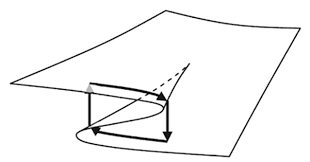
\includegraphics[width=\textwidth]{cusp}
    \end{minipage}
    
    \vfill
  \end{frame}

  \begin{frame}[t, c]{The cusp catastrophe}{\small Burger's equation}
    \vfill
    \large

    \begin{minipage}{.48\textwidth}
      \centering
      \underline{Convex conservation laws}

      \[
      \begin{aligned}
        & \dfrac{\partial u}{\partial t} + \nabla \cdot \bm{f} = 0 \\
        & u(\bm{x}, 0) = \varphi_0(\bm{x})
      \end{aligned}
      \]
    \end{minipage}%
    \hfill
    \begin{minipage}{.48\textwidth}
      \begin{itemize}
      \item $\bm{x}$ is 1-space variable,
      \item $\bm{f} = f(u)$, i.e. flux depends only on the state variable,
      \item $f(u)$ is $C^{\infty}$ and convex, i.e. $f^{\prime\prime}(u) > 0$.
      \end{itemize}
    \end{minipage}

    \vfill
  \end{frame}

  \begin{frame}[t, c]{The cusp catastrophe}{\small Burger's equation}
    \vfill
    \large

    \begin{minipage}{.48\textwidth}
      \centering

      \underline{Burger's equation}

      \begin{overprint}
        \onslide<1>
        \[
        \begin{aligned}
          & \dfrac{\partial u}{\partial t} + \dfrac{1}{2} \dfrac{\partial u^2}{\partial x} = 0 \\
          & u(x, 0) = \varphi_0(x)
        \end{aligned}
        \]

        \onslide<2>
        \[
        \begin{aligned}
          & \dfrac{\partial u}{\partial t} + u \dfrac{\partial u}{\partial x} = 0 \\
          & u(x, 0) = \varphi_0(x)
        \end{aligned}
        \]

      \end{overprint}
    \end{minipage}%
    \hfill
    \begin{minipage}{.48\textwidth}
      \centering
      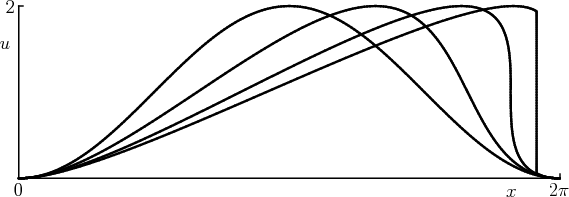
\includegraphics[width=\textwidth]{burgers_profile}
    \end{minipage}

    \vfill
  \end{frame}

  \begin{frame}[t, c]{The cusp catastrophe}{\small Burger's equation}
    \vfill
    \large
    
    The following equation is quite useful in solving this PDE.
    Let
    
    
    \[
    \begin{aligned}
      \dfrac{dx}{dt} & = u(x(t), t) \\
      x(0) & = x_0.
    \end{aligned}
    \]
    
    \medskip
    
    It is known as the \textbf{characteristic equation}.

    \vfill
  \end{frame}

  \begin{frame}[t, c]{The cusp catastrophe}{\small Burger's equation}
    \vfill
    \large

    Differentiating with respect to time $t$ yields
    
    \[
    \begin{aligned}
      \dfrac{d^2 x}{dt^2} & = \dfrac{\partial u}{\partial t} + u \dfrac{\partial u}{\partial x} \\
      & = 0.
    \end{aligned}
    \]
    
    Hence, $(x(t), t)$ is a straight line called a \textbf{characteristic}.
    Furthermore, the slope is constant and given by $u(x(t), t) = u(x_0, 0) = \varphi{x_0}$.

    \vfill
  \end{frame}

  \begin{frame}[t, c]{The cusp catastrophe}{\small Burger's equation}
    \centering
    \includegraphics[width=\textwidth]{burgers_characteristics}
  \end{frame}

}


{
  \setbeamercolor{background canvas}{bg=white}
  \begin{frame}[fragile]{}{}
    \vfill
    \flushright
    \Large
    \textbf{\color{black} Thank you for your attention}

    \large
    \textbf{\color{gray} Any question ?}
    \vfill
  \end{frame}
}

\end{document}
